%TC: macro \marginfootnote [other]
%TC: envir SCfigure [] other
%TC: macrocount beginSCfigure [figure]
\documentclass[11pt,twoside]{report}
\usepackage{preamble}
\setcounter{chapter}{2}
\graphicspath{{../img/}}
\def\includebibliography{}
\renewcommand{\chaptername}{Appendix}
\renewcommand{\thechapter}{\Alph{chapter}}

\begin{document}
\chapter{Computational geometry for the union of many spheres}
\label{appendix:computational-geometry}

\section{Introduction}

The two curvature measures, $C_{\partial\mathcal{L}}$ and $X_{\partial\mathcal{L}}$ (integrated mean and Gaussian curvatures respectively), are required for the morphological thermodynamics used extensively in the main text.
In this section we give details on their geometric construction to aid morphological calculations.
The relevant formulas for $C_{\partial\mathcal{L}}$ and $X_{\partial\mathcal{L}}$ in hard sphere systems have previously been given in references \cite{MeckeAA1994} and \cite{RothPRL2006}.
Here, we restate these formulas and extend them by computing their derivatives with respect to atomic coordinates.
This technical description is only likely to be of interest to those wishing to do morphological calculations of their own.
\todo{Tidy this appendix up so it is more thesis-y, and fix references!}

To briefly motivate these derivative calculations, we remind the reader that derivatives were used in the main text in the calculation of the free energy of local structures along the octahedron-tripyramid reaction path.
Gradients were required for this calculation, providing an analytic method (with perturbation theory) where the numerical method (thermodynamic integration) fails due the instability of intermediate points along the reaction path.
Full details of this method are given in Sec.\ \ref{SI:reaction-path}.
It is worth stating that the usefulness of gradient calculations extends beyond this one application.

The gradient gives the mean depletion forces between (nearby) particles within the bulk liquid, which is generally a quantity of interest in liquid state theories.
These solvation forces are useful for speeding up numerical minimisation procedures, and for describing the solvation forces for molecules and proteins in aqueous solution.
For the latter case one requires a solvent accessible surface $\partial{\mathcal{L}}$ which is composed of balls of varying radii; the formulas we present allow for this generalisation.

\section{Decomposing the solvent accessible surface into intersections}

For correlations in homogeneous liquids composed of identical balls, the curvatures must be computed across the solvent accessible surface $\partial\mathcal{L}$ where the enclosed volume is
\begin{equation*}
  \mathcal{L} = \cup_{i=1}^n B_\sigma(\vec{r}_i).
\end{equation*}
In order to keep the formulas as general as possible, we will consider a small generalisation of this surface where the spheres are of arbitrary radii, i.e.\
\begin{equation}\label{eq:generalised-volume}
  \mathcal{L} = \cup_{i=1}^n B_{\sigma_i}(\vec{r}_i),
\end{equation}
where $\sigma_i$ is the diameter of particle $i$.
One obtains the surface used in the main text by setting $\sigma_i = \sigma$ for all $i$.
Let $K^d \subseteq \mathbb{R}^d$ denote the space of \emph{polyconvex} subsets of $d$-dimensional Euclidean space.
By \emph{polyconvex} we mean subsets composed of a \emph{finite} union of convex subsets; this means the surfaces are well-behaved so standard geometric descriptions and intuitions apply.
By construction $\mathcal{L} \in \mathcal{K}^d$ and $\partial\mathcal{L} \in \mathcal{K}^{d-1}$.

If particle $i$ is on the surface of $\mathcal{L}$, i.e.
\begin{equation*}
  S_i %\equiv \partial B_\sigma(\vec{r}_i)
  \cap \partial\mathcal{L} \notin \emptyset %\in \mathcal{K}^{d-1}
\end{equation*}
where $S_i \equiv \partial B_{\sigma_i}(\vec{r}_i)$ is the spherical surface of particle $i$, then integrals over $\partial\mathcal{L}$ must carefully consider pieces $S_i$ and intersections $\bigcap_i S_i$ separately.
Intersections, e.g.\ $S_i \cap S_j$ for $i \ne j$, contribute zero area, but may have nonvanishing curvature; this is usually understood by considering the parallel surface $\partial(\mathcal{L}+B_\epsilon)$ in the limit as $\epsilon \to 0$.
Hard core interactions ensure pathological cases where spheres share a centre are excluded, so intersections of two spheres must result in a (one) lower dimensional manifold $S_i \cap S_j \in \mathcal{K}^{d-2}$.
It is straightforward to extend this argument to $n \le d$ intersections $\bigcap_{i=1}^{n} S_i \in \mathcal{K}^{d-n}$.
For $n = d$ intersections the solution is a zero-dimensional manifold, i.e.\ a point.

Intersections between $n > d$ spherical surfaces are possible in principle, but in practice they occur with vanishing probability once a system is thermalised.
To see this, consider an overlap of $n > d$ hard spheres.
By the above argument one can decompose the surface of the resulting structure into $k$-dimensional submanifolds where $0 \le k \le d$.
Higher order surface intersections $n>d$ requires multiple $n=d$ intersections to occur at the same point, which is overconstrained and occurs with measure zero.
Thus, the probability of finding points where $n > d$ spheres intersect occurs with measure zero.
This argument only applies because we considered the \emph{boundary} of the intersections; it is more common in the physics literature to consider the Mayer f-function (related to the Euler characteristic) of the intersection \emph{volumes}, where the measure is nonzero leading to slow convergence of the virial series \cite{Hansen2013}.
Despite having zero measure, there are cases where one would construct a geometry containing a higher order intersection so we will return to this topic in more detail in section \ref{sec:higher-order-intersections}.

In summary, for $d=3$ the surface $\partial\mathcal{L}$ contains the following submanifolds:
\begin{itemize}
\item $S_i \cap \partial\mathcal{L} \notin \emptyset$: a spherical cap from particle $i$.
\item $S_i \cap S_j \cap \partial\mathcal{L} \notin \emptyset$ for $i \ne j$: a line, specifically a circular arc.
\item Point $S_i \cap S_j \cap S_k \cap \partial\mathcal{L} \notin \emptyset$ for $i \ne j \ne k$: points where balls $i$, $j$, and $k$ intersect.
  3 intersecting spheres generally have 2 points of intersection, though usually only 1 of these coincides with the surface $\partial\mathcal{L}$ (the other is usually buried inside the volume $\mathcal{L}$).
\item Intersections of more than 3 surface spheres: occurs with vanishing probability in \emph{thermal} systems (see above).
\end{itemize}

In subsequent sections we will detail contributions to $C_{\partial\mathcal{L}}$ and $X_{\partial\mathcal{L}}$ (and their derivatives) from each of these intersections in $d=3$.
Note that for morphological thermodynamics one also requires the volume and surface area contributions, $V_\mathcal{L}$ and $A_{\partial\mathcal{L}}$, for which we do \emph{not} provide computational details as there is already a wealth of literature on this subject (notably Refs.\ \cite{EdelsbrunnerPNAS2003,BryantDCG2004}).
In particular, we found the algorithm in Ref.\ \cite{KleninJCC2011} to be fast and robust.
We extended their implementation to also compute integrated curvature measures, with the formulas given in subsequent sections.

\section{Integrated mean curvature}

\subsection{Notation}

In the main text we expressed the coordinates $\vec{r}^n \in \mathbb{R}^{3n}$ as the direct sum $\vec{r}^n = \vec{r}_1 \oplus \cdots \oplus \vec{r}_n$.
As each line contribution in \eqref{eq:integrated-curvature} depends on the positions of 2 central spheres, whose intersection forms a circle, together with 2 additional spheres whose intersections with the first two spheres creates terminating vertices for the circular arc.
Thus the line contribution depends on the positions of up to 4 particles, so the domain and image of the gradient is (potentially) 12-dimensional.
Fewer particles can be involved, and thus the dimension of the space is reduced, if:
\begin{itemize}
  \item $\theta_{l}^{(1)}$ and $\theta_{l}^{(2)}$ are formed by intersections with the same third particle, i.e.\ if both the solutions (points) to $S_1 \cap S_2 \cap S_i \; i \notin \{1, 2\}$ and the line joining them is on the surface $\partial\mathcal{S}$.
  In this case the space is 9-dimensional.
  \item $\phi_l = 2\pi$: the line forms a closed circle, uninterrupted by other particle intersections.
  In this case the space is 6-dimensional.
\end{itemize}
These cases are pathological and generally lines involve 4 particles so the space is 12-dimensional.

Given the large dimensionality we adopt the following notation to carefully distinguish each term in the space.
We recast the coordinates as the product space $\vec{r}^n \in \mathbb{R}^{n \times 3}$ so we can use the following notation for basis vectors:
\begin{equation*}
  \vec{e}_i^\alpha = \vec{e}_i \otimes \vec{e}_\alpha,
\end{equation*}
where $i \in \{1,\dots,n\}$ and $\alpha \in \{1,2,3\}$.
We use Roman indices to denote the particle number and Greek indices for the Cartesian component.

We use suffix notation where summation is assumed over repeated indices.
For example, we write the coordinates in summation convention as
\begin{equation*}
  \vec{r}^n = r_i^\alpha \vec{e}_i^\alpha := \sum_{i,\alpha} r_i^\alpha \vec{e}_i^\alpha.
\end{equation*}
One obtains the gradient from components of differentiation by summing over the basis vectors, as in
\begin{equation*}
  \vec{\nabla} f =
  \frac{\partial f}{\partial r_i^\alpha} \vec{e}_i^\alpha.
\end{equation*}
The latter expression can be used to determine gradients from the explicit forms of differentials given in subsequent sections.

\subsection{Problem}

The integrated mean curvature for the generalised solvent accessible surface $\partial\mathcal{L}$ where $\mathcal{L}$ is composed of spheres of differing radii as in \eqref{eq:generalised-volume} is given as \cite{RothPRL2006}
\begin{equation}\label{eq:integrated-curvature}
  C_{\partial\mathcal{L}} =
  \sum_{s \in S} \frac{A_s}{\sigma_s} -
  \sum_{l \in L} \frac{\phi_l R_l}{2} (\theta_l^{(1)} + \theta_l^{(2)}),
\end{equation}
where $A_s$ is the area of spherical cap $s$, $\phi_l$ is the angular length of the line $l$, $\phi_l R_l$ its arc length, and $\theta_l^{(1)}$ and $\theta_l^{(2)}$ are the angles between the spheres and the plane of intersection defined in Refs.\ \cite{ConnollyJAC1983,ConnollyJACS1985}, see Fig.\ \ref{fig:curvature-geometry}(a).
Algorithms already exist for computing the differential of the total area \cite{BryantDCG2004,KleninJCC2011}, so we do not need to consider the first term in \eqref{eq:integrated-curvature}.
This leaves only the line contributions for consideration.
The curvature contribution from a single line differentiates to give
\begin{equation}\label{eq:line-curvature-differential}
  \frac{\partial C_{\partial\mathcal{L}}}{\partial r_i^\alpha} =
  \sum_{s \in S} \frac{1}{\sigma_s}
  \frac{\partial A_s}{\partial r_i^\alpha} -
  \frac{1}{2} \sum_{l \in L} \left(
  \frac{\partial \phi_l}{\partial r_i^\alpha} R_l (\theta_l^{(1)} + \theta_l^{(2)}) +
  \phi_l \frac{\partial R_l}{\partial r_i^\alpha} (\theta_l^{(1)} + \theta_l^{(2)}) +
  (\phi_l R_l) \left(
  \frac{\partial \theta_l^{(1)}}{\partial r_i^\alpha} +
  \frac{\partial \theta_l^{(2)}}{\partial r_i^\alpha}
  \right)
  \right).
\end{equation}
In subsequent sections we will give explicit formulas for each differential in this expression.

%% The spherical caps contain the only area contributions, giving the area as
%% \begin{equation}
%%   A_{\partial\mathcal{L}} = \sum_i A[S_i]
%% \end{equation}

To get the curvature for the surface used in the main text one sets $\sigma_i = \sigma \; \forall \; i \in \{1 \dots n\}$.
In this limiting case the curvature \eqref{eq:integrated-curvature} simplifies to
\begin{equation*}
  C_{\partial\mathcal{L}} =
  \frac{A_{\partial\mathcal{L}}}{\sigma} -
  \sum_{l \in L} \frac{\phi_l R_l}{2} (\theta_l^{(1)} + \theta_l^{(2)}),
\end{equation*}
and many of the explicit expressions for $\phi_l$, $R_l$, $\theta_l^{(1)}$ and $\theta_l^{(2)}$ also simplify as will be seen in subsequent sections.

Note that in the computational algorithm which we use to compute $\partial\mathcal{L}$ (c.f.\ Ref.\ \cite{KleninJCC2011}) the symbol $\theta$ denotes the in-plane angle $\frac{\pi}{2} - \theta_l^{(\alpha)} \; \forall \; \alpha \in \{1,2\}$ is used instead in the construction of the surface, so formulas stated below must be adjusted in the implementation if this angle is used.

\begin{SCfigure}[b]
  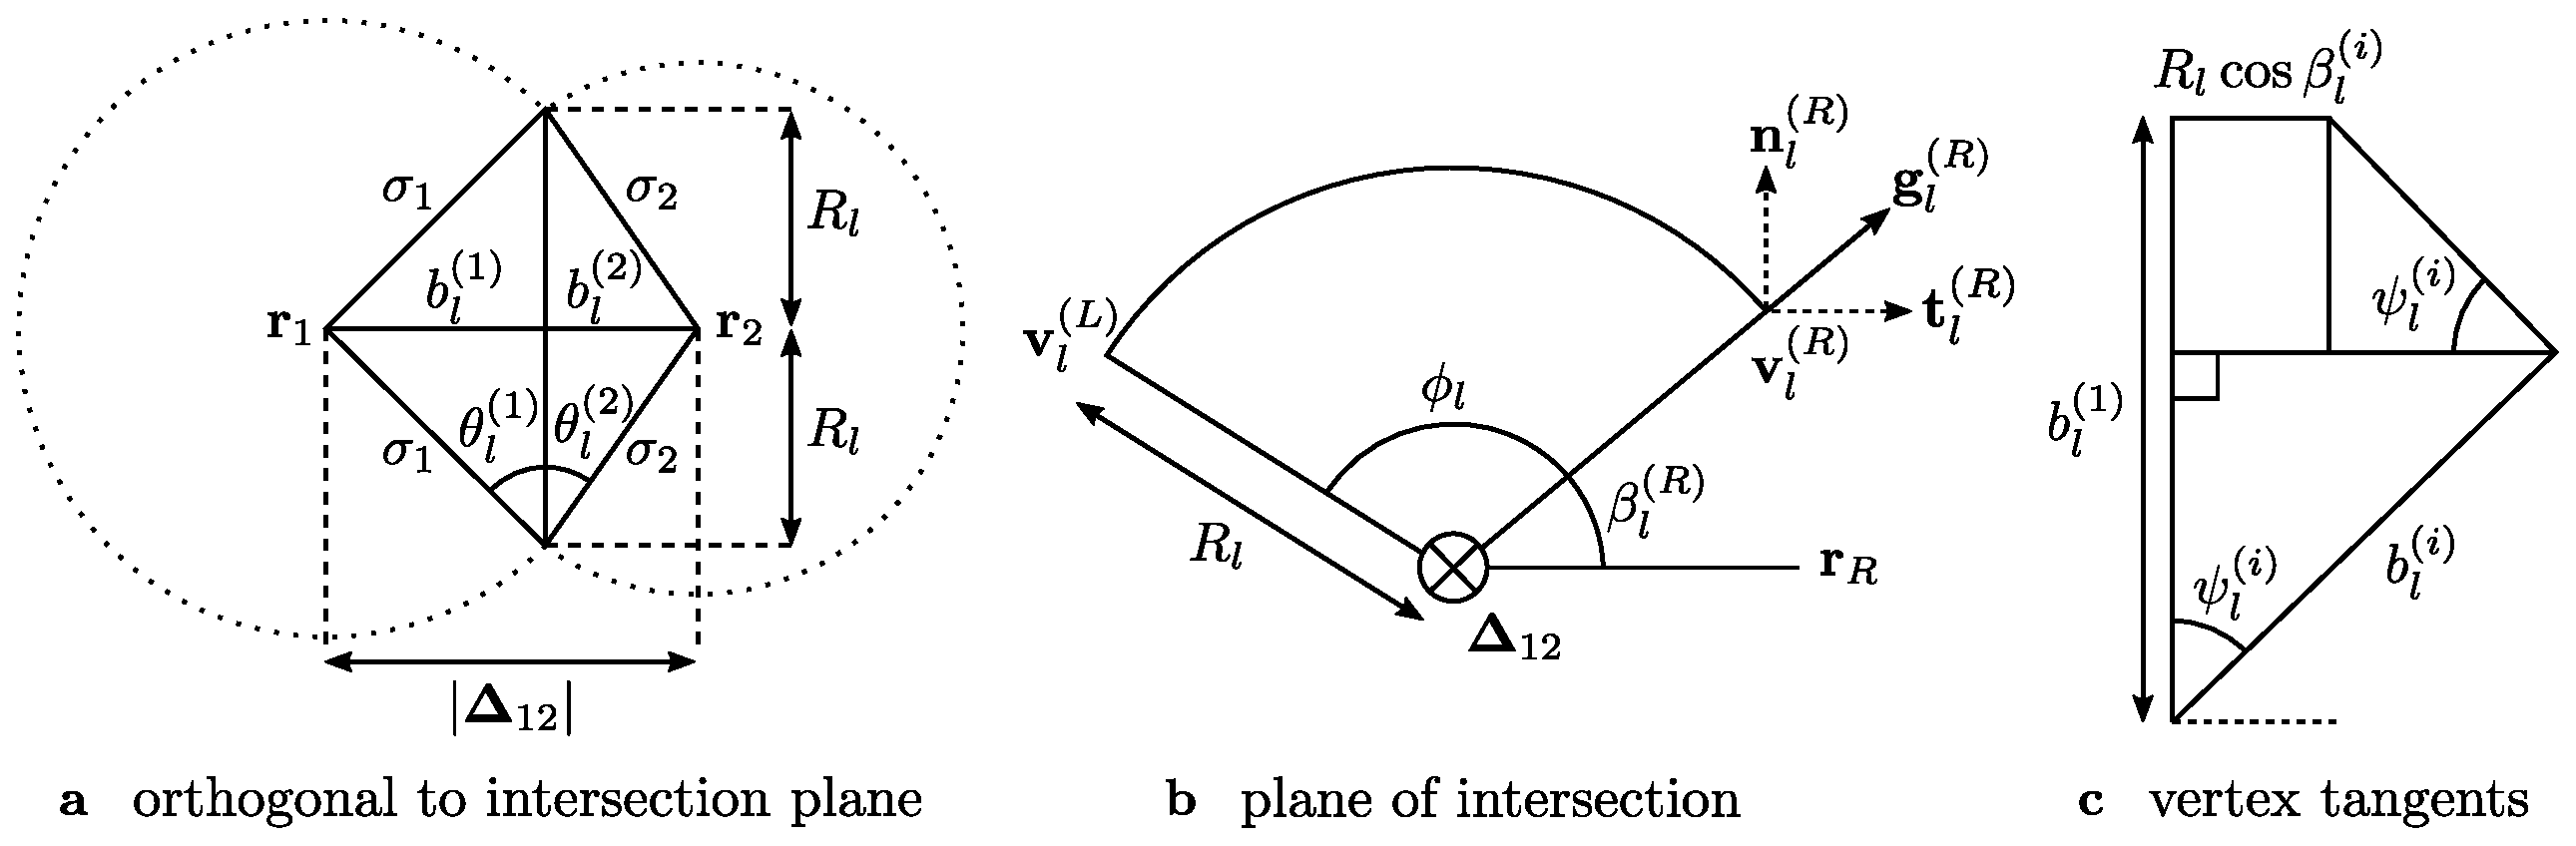
\includegraphics[width=\linewidth,outer]{curvature-geometry}
  \caption{Geometrical quantities involved in the calculation of line curvatures.}
  \label{fig:curvature-geometry}
\end{SCfigure}

\subsection{Particle separations}

The separation between two particle centers is
\begin{equation}
  \vec{\Delta}_{ij} = \vec{r}_i - \vec{r}_j
\end{equation}
which differentiates to
\begin{equation}
  \frac{\partial |\vec{\Delta}_{ij}|}{\partial r_k^\alpha} =
  \frac{r_i^\alpha - r_j^\alpha}{|\vec{\Delta}_{ij}|} (\delta_{ki} - \delta_{kj})
\end{equation}
where $\delta_{ij}$ is the Kronecker delta.

The basis vector for separations differentiates as
\begin{equation}
  \frac{\partial}{\partial r_k^\alpha}
  \left( \frac{\vec{\Delta}_{ij}}{|\vec{\Delta}_{ij}|} \right) =
  \frac{(\delta_{ki} - \delta_{kj}) \vec{e}_k^\alpha}{|\vec{\Delta}_{ij}|}
  - \frac{\vec{\Delta}_{ij}}{|\vec{\Delta}_{ij}|^2}
  \frac{\partial |\vec{\Delta}_{ij}|}{\partial r_k^\alpha}.
\end{equation}

\subsection{Quantities in the plane orthogonal to intersection}

We will label the particles whose intersection creates the circle of arc as 1 and 2 for convenience.
We consider the distances from these particles to the center of the circle as $b_l^{(1)}$ and $b_l^{(2)}$, see Fig.\ \ref{fig:curvature-geometry}(a).
Clearly $|\vec{\Delta}_{12}| = b_l^{(1)} + b_l^{(2)}$.
These distances form equilateral triangles with circle radius $R_l$ of hypotenuse $\sigma_i$ for $i \in \{1,2\}$.
This geometry is sketched in Fig.\ \ref{fig:curvature-geometry}a.
By Pythagoras' theorem we find the unknown distances as
\begin{align}
  R_l
  = \sigma_1 \, \cos{\theta_l^{(1)}}
  = \sigma_2 \, \cos{\theta_l^{(2)}}
  &= \frac{1}{2} \sqrt{
      2(\sigma_1^2 + \sigma_2^2) - |\vec{\Delta}_{12}|^2 -
      \left( \frac{\sigma_1^2 - \sigma_2^2}{|\vec{\Delta}_{12}|} \right)^2
    }, \\
  b_l^{(1)} = \sigma_1 \sin{\theta_l^{(1)}} &=
  \frac{ |\vec{\Delta}_{12}| + \frac{\sigma_1^2 - \sigma_2^2}{|\vec{\Delta}_{12}|} }{2}, \\
  b_l^{(2)} = \sigma_2 \sin{\theta_l^{(2)}} &=
  \frac{ |\vec{\Delta}_{12}| - \frac{\sigma_1^2 - \sigma_2^2}{|\vec{\Delta}_{12}|} }{2}.
\end{align}
The gradients of the angles between the planes are
\begin{subequations}
\begin{align}
  \frac{\partial \theta_l^{(1)}}{\partial r_i^\alpha} &=
  \frac{ 1 - \frac{\sigma_1^2 - \sigma_2^2}{|\vec{\Delta}_{12}|^2} }{2R_l}
  \frac{\partial |\vec{\Delta}_{12}|}{\partial r_i^\alpha}, \\
  \frac{\partial \theta_l^{(2)}}{\partial r_i^\alpha} &=
  \frac{ 1 + \frac{\sigma_1^2 - \sigma_2^2}{|\vec{\Delta}_{12}|^2} }{2R_l}
  \frac{\partial |\vec{\Delta}_{12}|}{\partial r_i^\alpha},
\end{align}
\end{subequations}
and the gradients of the distances are
\begin{subequations}
\begin{align}
  \frac{\partial R_l}{\partial r_i^\alpha} &=
  \frac{|\vec{\Delta}_{12}|}{4R_l}
  \left(
  \left( \frac{\sigma_1^2 - \sigma_2^2}{|\vec{\Delta}_{12}|} \right)^2 - 1 \right)
  \frac{\partial |\vec{\Delta}_{12}|}{\partial r_i^\alpha}, \\
  \frac{\partial b_l^{(1)}}{\partial r_i^\alpha} &=
  \frac{ 1 - \frac{\sigma_1^2 - \sigma_2^2}{|\vec{\Delta}_{12}|^2} }{2}
  \frac{\partial |\vec{\Delta}_{12}|}{\partial r_i^\alpha}, \\
  \frac{\partial b_l^{(2)}}{\partial r_i^\alpha} &=
  \frac{ 1 + \frac{\sigma_1^2 - \sigma_2^2}{|\vec{\Delta}_{12}|^2} }{2}
  \frac{\partial |\vec{\Delta}_{12}|}{\partial r_i^\alpha}.
\end{align}
\end{subequations}
As we must calculate the angles $\theta_l^{(1)}$ and $\theta_l^{(2)}$ and their derivatives for the curvature calculation, i.e.\ \eqref{eq:integrated-curvature} and \eqref{eq:line-curvature-differential}, a convenient form for these latter derivatives is
\begin{subequations}
\begin{align}
  \frac{\partial R_l}{\partial r_i^\alpha} &
  = - b_l^{(1)} \frac{\partial\theta_l^{(1)}}{\partial r_i^\alpha}
  = - b_l^{(2)} \frac{\partial\theta_l^{(2)}}{\partial r_i^\alpha}, \\
  \frac{\partial b_l^{(1)}}{\partial r_i^\alpha} &=
  R_l \frac{\partial\theta_l^{(1)}}{\partial r_i^\alpha}, \\
  \frac{\partial b_l^{(2)}}{\partial r_i^\alpha} &=
  R_l \frac{\partial\theta_l^{(2)}}{\partial r_i^\alpha}.
\end{align}
\end{subequations}

The expressions in this section are the only quantities which explicitly depend on the sizes of the spheres $\sigma_i$, so we see how it is straightforward to consider the more general surface composed of arbitrarily sized spheres.
The above formulas are simplified if spheres are of equal sizes i.e.\ $\sigma_i = \sigma$ (as in the main text) leading to vanishing of $\sigma_1^2 - \sigma_2^2$ terms.

\subsection{Angular length}

To complete the derivatives in \eqref{eq:line-curvature-differential} we need an explicit expression for the gradient of the angular separation $\phi_l$.
In general, the line consists of an arc along a circle of radius $R_l$, which terminates at the vertices.
%It is possible for lines to not terminate at vertices, however we do not need to consider this special case as it occurs where $\phi_l = 2\pi$ is a constant so the gradient is zero and can be ignored.

We consider the 2d plane containing the intersection $S_1 \cap S_2$.
The center of the intersection circle is
\begin{equation}
  \vec{c}_l
  = \vec{r}_1 + b_l^{(1)} \frac{\vec{\Delta}_{12}}{|\vec{\Delta}_{12}|}
  = \vec{r}_2 - b_l^{(2)} \frac{\vec{\Delta}_{12}}{|\vec{\Delta}_{12}|}.
\end{equation}
The plane of intersection is seen by looking along $\vec{\Delta}_{12}$, making the arc $\phi_l R_l$ perfectly circular, shown in Fig.\ \ref{fig:curvature-geometry}b.
By convention we choose the arc to be a clockwise migration from a `left' vertex to a `right' vertex, which we label $v_l^{(L)}$ and $v_l^{(R)}$ accordingly.
These vertices form at 3-particle intersections, so we will use the suffixes $L$ and $R$ to indicate the 3rd particle index (distinct from 1 and 2) where appropriate.
We write the vertex coordinates as
\begin{equation}
  \vec{v}_l^{(i)} = \vec{c}_l + R_l \, \vec{g}_l^{(i)} \qquad i \in \{L,R\},
\end{equation}
where the unit vectors are
\begin{equation}
  \vec{g}_l^{(i)} =
  \frac
  {\vec{v}_l^{(i)} - \vec{c}_l}
  {|\vec{v}_l^{(i)} - \vec{c}_l|}
  \qquad i \in \{L,R\}.
\end{equation}
The unit vectors for the `right' component are sketched in Fig.\ \ref{fig:curvature-geometry}b.
The central angle is thus defined as the angle (going clockwise) between these unit vectors, i.e.
\begin{equation}
  \cos{\phi_l} = \vec{g}_l^{(L)} \cdot \vec{g}_l^{(R)},
\end{equation}
which after differentiation gives
\begin{equation}
  \frac{\partial \phi_l}{\partial r_i^\alpha} =
  - \frac
  {\frac{\partial \vec{g}_l^{(L)}}{\partial r_i^\alpha} \cdot \vec{g}_l^{(R)} +
   \vec{g}_l^{(L)} \cdot \frac{\partial \vec{g}_l^{(R)}}{\partial r_i^\alpha}}
  {\sin{\phi_l}}.
\end{equation}
So we need explicit expressions for vectors $\vec{g}_l^{(L)}$ and $\vec{g}_l^{(R)}$ and their derivatives to proceed.

We decompose the vertex unit vectors into the following Cartesian basis:
\begin{equation}\label{eq:vertex-unit-vector}
  \vec{g}_l^{(i)} =
  \cos{\beta_l^{(i)}} \, \vec{t}_l^{(i)} + \sin{\beta_l^{(i)}} \, \vec{n}_l^{(i)}
  \qquad i \in \{L,R\},
\end{equation}
where $\vec{t}_l^{(i)}$ is the vector tangent to the plane spanned by particles $\{1,2,i\}$ and $\vec{n}_l^{(i)}$ is normal to this plane.
If $\psi_l^{(i)}$ is the angle $\angle 1i2$, that is
\begin{equation}\label{eq:cos-psi}
  \cos{\psi_l^{(i)}} =
  \frac{\vec{\Delta}_{12} \cdot \vec{\Delta}_{1i}}
  {|\vec{\Delta}_{12}||\vec{\Delta}_{1i}|}
  \qquad i \in \{L,R\}
\end{equation}
then these basis vectors take the form
\begin{subequations}\label{eq:vertex-unit-vector-basis}
\begin{align}
  \vec{n}_l^{(L)} &=
  %\frac{\vec{e}_c \times \vec{e}_l}{|\vec{e}_c \times \vec{e}_l|} =
  \frac{1}{\sin{\psi_l^{(L)}}}
  \frac{\vec{\Delta}_{12} \times \vec{\Delta}_{1L}}
  {|\vec{\Delta}_{12}||\vec{\Delta}_{1L}|}, \\
  \vec{n}_l^{(R)} &=
  %\frac{\vec{e}_r \times \vec{e}_c}{|\vec{e}_r \times \vec{e}_c|} =
  \frac{1}{\sin{\psi_l^{(R)}}}
  \frac{\vec{\Delta}_{1R} \times \vec{\Delta}_{12}}
  {|\vec{\Delta}_{1R}||\vec{\Delta}_{12}|}, \\
  \vec{t}_l^{(L)} &=
  \frac{\vec{n}_l^{(L)} \times \vec{\Delta}_{12}}{|\vec{\Delta}_{12}|}, \\
  \vec{t}_l^{(R)} &=
  \frac{\vec{\Delta}_{12} \times \vec{n}_l^{(R)}}{|\vec{\Delta}_{12}|}.
\end{align}
\end{subequations}
Finally, from Fig.\ \ref{fig:curvature-geometry}c we have
\begin{equation}
  b_l^{(i)} \sin{\beta_l^{(i)}} - R_l \cos{\beta_l^{(i)}}
  = \frac{b_l^{(1)} - b_l^{(i)} \cos{\psi_l^{(i)}}}{\tan{\psi_l^{(i)}}}
  \qquad i \in \{L,R\},
\end{equation}
giving
\begin{equation}\label{eq:cos-beta}
  \vec{g}_l^{(i)} \cdot \vec{t}_l^{(i)} = \cos{\beta_l^{(i)}} =
  \frac{1}{R_l} \left(
    b_l^{(i)} \sin{\psi_l^{(i)}}
    + \frac{b_l^{(i)} \cos{\psi_l^{(i)}} - b_l^{(1)}}{\tan{\psi_l^{(i)}}}
  \right)
  \qquad i \in \{L,R\}.
\end{equation}

With explicit expressions for all of the vectors involved in the arc, the only remaining step is to differentiate.
First, we differentiate the vertex unit vectors \eqref{eq:vertex-unit-vector} in the basis defined by \eqref{eq:vertex-unit-vector-basis} to obtain
\begin{equation}
  \frac{\partial \vec{g}_l^{(j)}}{\partial r_i^\alpha} =
  \frac{\vec{g}_l^{(j)} \times \vec{\Delta}_{12}}{|\vec{\Delta}_{12}|} \,
  \frac{\partial \beta_l^{(j)}}{\partial r_i^\alpha} +
  \cos{\beta_l^{(j)}} \,
  \frac{\partial \vec{t}_l^{(j)}}{\partial r_i^\alpha} +
  \sin{\beta_l^{(j)}} \,
  \frac{\partial \vec{n}_l^{(j)}}{\partial r_i^\alpha}
  \qquad j \in \{L,R\}.
\end{equation}
Second, we take the derivatives of the basis vectors themselves \eqref{eq:vertex-unit-vector-basis} giving
\begin{subequations}
\begin{align}
  \frac{\partial \vec{n}_l^{(L)}}{\partial r_i^\alpha} &=
  \frac{\vec{e}_{c,j} \times \vec{e}_l + \vec{e}_c \times \vec{e}_{l,j}}{\sin{\psi_l}}
  - \frac{\cos{\psi_l}}{\sin{\psi_l}} \psi_{l,j} \, \vec{n}_l, \\
  \frac{\partial \vec{n}_l^{(R)}}{\partial r_i^\alpha} &=
  \frac{\vec{e}_{r,j} \times \vec{e}_c + \vec{e}_r \times \vec{e}_{c,j}}{\sin{\psi_r}}
  - \frac{\cos{\psi_r}}{\sin{\psi_r}} \psi_{r,j} \, \vec{n}_r,
\end{align}
\end{subequations}
Finally, we differentiate the angles from \eqref{eq:cos-psi} and \eqref{eq:cos-beta} to get
\begin{subequations}
\begin{align}
 \frac{\partial \beta_l^{(j)}}{\partial r_i^\alpha} &=
  \frac{
  \frac{\partial R_l}{\partial r_i^\alpha}
  \cos{\beta_l^{(j)}} -
  \frac{\partial}{\partial r_i^\alpha}
  \left( R_l \cos{\beta_l^{(j)}} \right)}
  {R_l \sin{\beta_l^{(j)}}}, \\
 \frac{\partial}{\partial r_i^\alpha}
  \left( R_l \cos{\beta_l^{(j)}} \right) &=
  \frac{1}{\sin{\psi_l^{(j)}}}
  \frac{\partial b_l^{(j)}}{\partial r_i^\alpha}
  - \frac{1}{\tan{\psi_l^{(j)}}}
  \frac{\partial b_l^{(1)}}{\partial r_i^\alpha}
  - \frac{b_l^{(j)} \cos{\psi_l^{(j)}} - b_l^{(1)}}
  {\sin^2{\psi_l^{(j)}}}
  \frac{\partial \psi_l^{(j)}}{\partial r_i^\alpha}, \\
  \frac{\partial \psi_l^{(j)}}{\partial r_i^\alpha} =
  -\frac{1}{\sin\psi_l^{(j)}} \frac{\partial(\cos{\psi_l^{(j)}})}{\partial r_i^\alpha} &=
  -\frac{1}{\sin\psi_l^{(j)}}
  \left(
  \frac{\partial}{\partial r_i^\alpha}
  \left( \frac{\vec{\Delta}_{12}}{|\vec{\Delta}_{12}|} \right) \cdot
  \frac{\vec{\Delta}_{1j}}{|\vec{\Delta}_{1j}|}
  +
  \frac{\vec{\Delta}_{12}}{|\vec{\Delta}_{12}|} \cdot
  \frac{\partial}{\partial r_i^\alpha}
  \left( \frac{\vec{\Delta}_{1j}}{|\vec{\Delta}_{1j}|} \right)
  \right),
\end{align}
\end{subequations}
for $j \in \{L,R\}$ in each expression.

\section{Integrated Gaussian curvature}

$\partial\mathcal{L}$ forms a closed two-dimensional surface, so by the Gauss-Bonnet theorem \eqref{eq:gauss-bonnet} we find $X$ is a topological constant of the surface.
Thus, the derivative of $X$ is zero everywhere except at pathological points where a topological change in the surface occurs.
In practice this happens when a cavity larger than a particle size forms inside the structure, or when a particle dissociates; being interested in \emph{compact} local structures, we can exclude both of these scenarios from consideration.
Thus, for all local structures $\chi=2$, and the gradient of $X$ is zero everywhere.

Under the above assumptions we do not need to compute $X_{\partial\mathcal{L}}$, but nevertheless it is convenient to do so in order to check the correctness of the algorithm:
\begin{equation}
  X_{\partial\mathcal{L}} =
  -\sum_{l \in L} \phi_l (\sin{\theta_l^{(1)}} + \sin{\theta_l^{(2)}}) +
  \sum_{(i,j,k) \in V} \Omega_{ijk}
\end{equation}
where $\Omega_{ijk}$ is the solid angle spanned by the 3-vectors at vertex $S_i \cap S_j \cap S_k$ \cite{MeckeAA1994}.
The condition that this sum must produce the same result as \eqref{eq:gauss-bonnet} provides a useful check of the numerics.

\section{Intersections of more bodies: possible caveats with quenched geometries}
\label{sec:higher-order-intersections}

A common task with computer simulations is to quench a geometry to find the minimal (or \emph{inherent}) energy structure.
Quenched geometries are inherently athermal so the argument above that intersections of $n>d$ spheres should occur with vanishing probability does not apply; it is common to find intersections of 4 or more particles at the surface in $d=3$ \emph{after a quench}.
To investigate quenched geometries one must properly treat such intersections, as we will demonstrate below with an illustrative example.

An example of these intersections in $d=3$ occurs where 4 particles are arranged in a perfect square (as in e.g.\ any outer face of the body-centered cubic unit cell).
This special geometry corresponds to a bifurcation point in configuration space, where two pairs of surface vertices are simultaneously created and annihilated.
The gradient is not continuous at these points \emph{with respect to the atomic coordinates}, as the continuity of the morphological free energy is only guaranteed with respect to the set $\mathcal{L}$ according to the Hausdorff metric.
In atomic coordinates derivatives can contain poles and step discontinuities.

As the example above illustrates, the gradient is not well defined at pathological points where many spheres intersect.
It is thus impossible to quench these geometries using standard algorithms (which assume smooth functions) and perturbation theories (e.g.\ the harmonic approximation for the free energy) will fail.
A proper treatment of these cases would be required for an investigation of quenched geometries.
In this work we have avoided these considerations primarily by restricting ourselves to geometries thermalised using a Monte-Carlo algorithm (Figures \ref{fig:structure-populations} and \ref{fig:reaction} in the main text).
Construction of the reaction path of $n=6$ particles necessitates an analytic method which uses a quenched geometry, however the geometries for $n=6$ are not pathological so no special consideration is needed.

\ifdefined\includebibliography
  \printbibliography
\fi

\end{document}
